\documentclass[10pt]{beamer}
\usepackage{my_style}

%%%%%%%%%%%%%%%%%%%%%%%%%%%%%%%%%%%%%%%%%%%%%%%%%%%%%%%%%%%%%%%%%%%%%%%%
\title[Math/CS 375]{Lecture 05 - A}
\subtitle{Linear Algebra Fundamentals}

\begin{document}
% -------------------------------------------------
\begin{frame}
  \titlepage
\end{frame}
% -------------------------------------------------

\begin{frame}{Goals}
We will answer these questions:\\[3mm]
\begin{itemize}
    \item How do you multiply a matrix and a vector? 
    \item What is the difference between the row and column views of the multiplication $Ax$?
    \item What is a linear system? 
    \item What does it mean for a matrix to be invertible? 
    \item What is the fundamental theorem of linear algebra?
\end{itemize}
\end{frame}

%%%%%%%%%%%%%%%%%%%%%%%%%%%%%%%%%%%%%%%%%%%%%%%%%%%%%%%%%%%%%
\sectionframe{Notation}
%%%%%%%%%%%%%%%%%%%%%%%%%%%%%%%%%%%%%%%%%%%%%%%%%%%%%%%%%%%%%
\begin{frame}[fragile]
\frametitle{Matrix Notation}
\begin{itemize}
\item A \textbf{matrix} $A \in \mathbb{R}^{m\times n}$  has the form 
\begin{equation*}
    A = \begin{bmatrix} a_{11} & a_{12} & \cdots & a_{1n} \\
                        a_{21} & a_{22} &        & a_{2n} \\
                        \vdots &        & \ddots & \vdots \\
                        a_{m1} &        & \cdots & a_{mn} \\
        \end{bmatrix}
\end{equation*}
\vfill 

\item The entry in row $i$ and column $j$ is denoted
\begin{equation*}
    a_{ij}.
\end{equation*}
\vfill 
\item May also write $(A)_{ij}$
\vfill 
\end{itemize}
\end{frame}

%%%%%%%%%%%%%%%%%%%%%

\begin{frame}[fragile]
\frametitle{Vector Notation}
\begin{itemize}
    \item A \textbf{vector} $v \in \mathbb{R}^n$ with $n$ components has the form
\begin{equation*}
    v = \begin{bmatrix} v_{1}  \\
                        v_{2}  \\
                        \vdots  \\
                        v_{n}  \\
        \end{bmatrix}
\end{equation*}

\item The $i^{th}$ element in $v$ is denoted 
    $$v_i$$ 

% \item We will not use $\vec{v}$ nor $\textbf{v}$

\item Vectors are always assumed to be \textit{columns} $(n\times 1)$
\vfill
\item We can \textbf{transpose} a vector to make it into a \textit{row}
    $$ v' = v^T= \begin{bmatrix} v_{1} & v_{2} & \cdots & v_{n} \end{bmatrix}$$

\end{itemize}
\end{frame}


%%%%%%%%%%%%%%%%%%%%%%%%%%%%%%%%%%%%%%%%%%%%%%%%%%%%%%%%%%%%%%%%%%%%%%%%
\begin{frame}{Rows and Columns}

\begin{minipage}[t]{0.45\textwidth}
As a collection of column vectors
\begin{equation*}
    A =
    \begin{bmatrix}\left. \begin{matrix} \\ \\ a_{(1)}  \\ \\ \\ \end{matrix}\right|
                   \left. \begin{matrix} \\ \\ a_{(2)}  \\ \\ \\ \end{matrix}\right|
                   \left. \begin{matrix} \\ \\ {\cdots\ } \\ \\ \\ \end{matrix}\right|
                          \begin{matrix} \\ \\ a_{(n)}  \\ \\ \\ \end{matrix}\negthickspace
    \end{bmatrix}
\end{equation*}
\end{minipage}
\hspace{3ex}
\begin{minipage}[t]{0.45\textwidth}
As a collection of row vectors
\begin{equation*}
    A =
    \begin{bmatrix}\begin{matrix} & & a'_{(1)}& & & \end{matrix} \\
                   \dfrac{\makebox[1.2in]{}}{\makebox[1.2in]{}} \\
                   \begin{matrix} & & a'_{(2)}& & & \end{matrix} \\
                   \dfrac{\makebox[1.2in]{}}{\makebox[1.2in]{}} \\
                   \begin{matrix} & & \vdots & & & \end{matrix} \\
                   \dfrac{\makebox[1.2in]{}}{\makebox[1.2in]{}} \\
                   \begin{matrix} & & a'_{(m)}& & & \end{matrix} \\
    \end{bmatrix}
\end{equation*}
\end{minipage}
\begin{itemize}
    \item We may view matrices as a collection of columns or rows
\end{itemize}
\end{frame}


% scalar multiplication 

\begin{frame}{Basic Operations}


\begin{block}{Vector Addition}
Add two vectors $w=u+v$
$$
    w_i = u_i+v_i
$$    
\end{block}


\begin{block}{Scalar multiplication}
Multiply a vector $v$ by a scalar $\alpha \in \mathbb{R}$  $w = \alpha v$
$$
    w_i = \alpha \,v_i
$$
\end{block}


\define{Linear Combination}{
A \textbf{linear combination} of vectors
$u_1,u_2,\ldots,u_k \in \mathbb{R}^n$ is an expression
\[
    \alpha_1u_1+\alpha_2u_2+\cdots+\alpha_ku_k
    = \sum_{j=1}^k \alpha_j u_j,
\]
where $\alpha_1,\ldots,\alpha_k \in \mathbb{R}$ are scalars.
}
\end{frame}


%%%%%%%%%%%%%%%%%%%%%%%%%%%%%%%%%%%%%%%%%%%%%%%%%%%%%%%%%%%%%%%%%%%%
\sectionframe{Norms}
%%%%%%%%%%%%%%%%%%%%%%%%%%%%%%%%%%%%%%%%%%%%%%%%%%%%%%%%%%%%%%%%%%%%

\begin{frame}{Vector Norm}

\begin{itemize}
    \item For a scalar $x\in\mathbb{R}$, the absolute value $|x|$ measures its size.
    \item For a vector $v\in\mathbb{R}^n$, we use a \textbf{norm} to measure its size.
\end{itemize}

\define{Euclidean Norm}{
The \textbf{Euclidean norm} (or $2$-norm) of
\[
v=
\begin{bmatrix}
v_1\\v_2\\ \vdots\\v_n
\end{bmatrix}
\]
is
\[
\boxed{
\|v\|_2
=
\sqrt{v_1^2+v_2^2+\cdots+v_n^2}
}
\]
}

\keyidea{
The norm $\|v\|_2$ is the length of the vector $v$.
}
\end{frame}

% -------------- 
\begin{frame}{Vector Norm}{Geometric Interpretation}

\begin{itemize}
\item Consider the vectors
\[
v=
\begin{bmatrix}
3\\4
\end{bmatrix}
\qquad \text{and} \qquad
w=2v=
\begin{bmatrix}
6\\8
\end{bmatrix}.
\]

\begin{center}
\begin{tikzpicture}[scale=0.38]
    \draw[->] (-0.5,0) -- (7,0) node[right] {$x_1$};
    \draw[->] (0,-0.5) -- (0,9) node[above] {$x_2$};

    \draw[dashed] (3,0) -- (3,4);
    \draw[dashed] (0,4) -- (3,4);

    \draw[->, very thick] (0,0) -- (3,4)
        node[midway, above left] {$v$};

    \node[below] at (3,0) {$3$};
    \node[left] at (0,4) {$4$};
\end{tikzpicture}
\hspace{1cm}
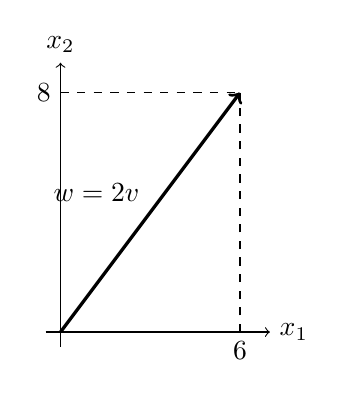
\begin{tikzpicture}[scale=0.38]
    \draw[->] (-0.5,0) -- (7,0) node[right] {$x_1$};
    \draw[->] (0,-0.5) -- (0,9) node[above] {$x_2$};

    \draw[dashed] (6,0) -- (6,8);
    \draw[dashed] (0,8) -- (6,8);

    \draw[->, very thick] (0,0) -- (6,8)
        node[midway, above left] {$w=2v$};

    \node[below] at (6,0) {$6$};
    \node[left] at (0,8) {$8$};
\end{tikzpicture}
\end{center}

\item Notice their norms:
\[
    \|v\|_2=\sqrt{3^2+4^2}=5,
    \qquad
    \|w\|_2=\sqrt{6^2+8^2}=10.
\]
\end{itemize}

\end{frame}

%%%%%%%%%%%%%%%%%%%%%%%%%%%%%%%%%%%%%%%%%%%%%%%%%%%%%%%%%%%%%%%%%%%%%%%%
\begin{frame}{Scaling a Vector}

\begin{itemize}
    \item  Suppose we multiply a vector by a scalar:
\[
w=\alpha v.
\]

\item  What happens to its length?

\begin{align*}
\|\alpha v\|_2
&=
\sqrt{(\alpha v_1)^2+\cdots+(\alpha v_n)^2}\\
&=
|\alpha|
\sqrt{v_1^2+\cdots+v_n^2}\\
&=
\boxed{|\alpha|\|v\|_2}.
\end{align*}

\vfill

\item Length is scaled by $\alpha $
\end{itemize}

\onslide<2>{
\question{
How can we scale a vector to have length $1$
without changing its direction?
}
}

\end{frame}

%%%%%%%%%%%%%%%%%%%%%%%%%%%%%%%%%%%%%%%%%%%%%%%%%%%%%%%%%%%%%%%%%%%%%%%%
\begin{frame}{Normalization}

\define{Normalized Vector}{
For a nonzero vector $v$, its \textbf{normalized vector} is
\[
\widehat{v}
=
\frac{1}{\|v\|_2}v.
\]
}


\onslide<2->{
Its length is
\[
\|\widehat{v}\|_2
=
\left\|
\frac{1}{\|v\|_2}v
\right\|_2
=
\frac{1}{\|v\|_2}\|v\|_2
=
1.
\]

\keyidea{
Normalization changes the length of a vector to $1$
while preserving its direction.
}
}

\end{frame}

%%%%%%%%%%%%%%%%%%%%%%%%%%%%%%%%%%%%%%%%%%%%%%%%%%%%%%%%%%%%%%%%%%%%%%%%
\begin{frame}{Normalization}{Example}

\begin{example}
Normalize the vector
\[
v=
\begin{bmatrix}
3\\4
\end{bmatrix}.
\]
\end{example}

First, compute its norm:
\[
\|v\|_2
=
\sqrt{3^2+4^2}
=
5.
\]

Therefore,
\[
\widehat{v}
=
\frac{v}{\|v\|_2}
=
\frac{1}{5}
\begin{bmatrix}
3\\4
\end{bmatrix}
=
\begin{bmatrix}
3/5\\4/5
\end{bmatrix}.
\]

Check:
\[
\|\widehat{v}\|_2
=
\sqrt{\left(\frac35\right)^2+\left(\frac45\right)^2}
=
1.
\]

\end{frame}

%%%%%%%%%%%%%%%%%%%%%%%%%%%%%%%%%%%%%%%%%%%%%%%%%%%%%%%%%%%%%%%%%%%%%%%%
\sectionframe{Linear Algebra Multiplication}
%%%%%%%%%%%%%%%%%%%%%%%%%%%%%%%%%%%%%%%%%%%%%%%%%%%%%%%%%%%%%%%%%%%%%%%%
\begin{frame}{Product of Vectors}    

\begin{block}{Inner Product}
The \textbf{inner product} (row $\times$ column) results in a scalar 
$$
    u'v =  \begin{bmatrix} u_1 & u_2 & \cdots & u_n \end{bmatrix}
    \begin{bmatrix} v_{1}  \\
                v_{2}  \\
                \vdots  \\
                v_{n}  \\
     \end{bmatrix} = 
     \sum\limits_{i=1}^{n} u_i v_i
$$
\end{block}

\begin{block}{Outer Product}
For $u\in\mathbb{R}^m$ and $v\in\mathbb{R}^n$, the
\textbf{outer product} (column $\times$ row) is an
$m\times n$ matrix:
\[
uv'=
\begin{bmatrix}
    u_1\\u_2\\\vdots\\u_m
\end{bmatrix}
\begin{bmatrix}
    v_1 & v_2 & \cdots & v_n
\end{bmatrix}
=
\begin{bmatrix}
    u_1v_1 & u_1v_2 & \cdots & u_1v_n\\
    u_2v_1 & u_2v_2 & \cdots & u_2v_n\\
    \vdots & \vdots & \ddots & \vdots\\
    u_mv_1 & u_mv_2 & \cdots & u_mv_n
\end{bmatrix}.
\]
\end{block}
\end{frame}

%%%%%%%%%%%%%%%%%%%%%%%%%%%%%%%%%%%%%%%%%%%%%%%%%%%%%%%%%%%%%%%%%%%%%%%%
\begin{frame}{Matrix--Vector Product}
\begin{itemize}
\item Multiply a matrix $A\in\mathbb{R}^{m\times n}$
by a vector $x\in\mathbb{R}^n$
    \begin{equation*}
        Ax = \begin{bmatrix} a_{11} & a_{12} & \cdots & a_{1n} \\
                        a_{21} & a_{22} & \cdots & a_{2n} \\
                               &        &        &        \\
                        \vdots & \vdots &        & \vdots \\
                               &        &        &        \\
                        a_{m1} & a_{m2} & \cdots & a_{mn}
        \end{bmatrix}
        \begin{bmatrix} x_1 \\ x_2 \\ \vdots \\ x_n \end{bmatrix}
    \end{equation*}
    \item Inner dimensions must agree
    $$
    \begin{array}{cccc}
                A       &        x        & = & b \\[3pt]
        [\matdim{m}{n}] & [\matdim{n}{1}] & = & [\matdim{m}{1}]
    \end{array}$$
\end{itemize}
\end{frame}

%%%%%%%%%%%%%%%%%%%%%%%%%%%%%%%%%%%%%%%%%%%%%%%%%%%%%%%%%%%%%%%%%%%%%%%%
\begin{frame}{Two Ways of Viewing Matrix-Vector Product}

\begin{itemize}
\item The Row View treats $b$ as a vector of inner products
\begin{equation*}
\begin{bmatrix}\begin{matrix} & & a'_{(1)}& & & \end{matrix} \\
       \dfrac{\makebox[1.2in]{}}{\makebox[1.2in]{}} \\
       \begin{matrix} & & \vdots & & & \end{matrix} \\
       \dfrac{\makebox[1.2in]{}}{\makebox[1.2in]{}} \\
       \begin{matrix} & & a'_{(m)}& & & \end{matrix}
\end{bmatrix}
\begin{bmatrix} x_1 \\ x_2 \\ \vdots \\ x_n \end{bmatrix} = 
\begin{bmatrix} b_1 \\ \vdots \\ b_m \end{bmatrix}
\end{equation*}

\item The Column View treats $b$ as a linear combination of the columns of $A$

\begin{equation*}
\begin{bmatrix}\left. \begin{matrix} \\ \\ a_{(1)}  \\ \\ \\ \end{matrix}\right|
       \left. \begin{matrix} \\ \\ a_{(2)}  \\ \\ \\ \end{matrix}\right|
       \left. \begin{matrix} \\ \\ {\cdots\ } \\ \\ \\ \end{matrix}\right|
              \begin{matrix} \\ \\ a_{(n)}  \\ \\ \\ \end{matrix}\negthickspace
\end{bmatrix}
\begin{bmatrix} x_1 \\ x_2 \\ \vdots \\ x_n \end{bmatrix}
=
\begin{bmatrix}  \\  \\ b \\  \\  \\ \end{bmatrix}
\end{equation*}

\end{itemize}   
\end{frame}
%%%%%%%%%%%%%%%%%%%%%%%%%%%%%%%%%%%%%%%%%%%%%%%%%%%%%%%%%%%%%%%%%%%%%%%%
\begin{frame}{In the Row View}
\begin{itemize}
    \item Treat $A$ as a collection of rows
\begin{center}
    \pgfimage[height=4cm]{./figs/matrixVectorRows}
\end{center}

\item Formula for the product is 
$$ y_i = a'_{(i)}x = \sum_{j=1}^n a_{ij}x_j$$
\end{itemize}

\end{frame}

%%%%%%%%%%%%%%%%%%%%%%%%%%%%%%%%%%%%%%%%%%%%%%%%%%%%%%%%%%%%%%%%%%%%%%%%
\begin{frame}{Row View Example}

\begin{example}
Calculate the product $Ax$ in the row view
\begin{equation*}
    \left[\negthickspace
          \begin{array}{rrr}  5 &  1  &  0    \\
                              0 &  4  & -2     \\
                              1 &  2  &  3    \end{array}\negthickspace\right]
    \left[\negthickspace
          \begin{array}{r}  2 \\  0  \\  -3  \end{array}\negthickspace\right]
\end{equation*}
\end{example}

Take the inner product of each row with the vector
\begin{equation*}
    \hfill
    = \left[\negthickspace
          \begin{array}{rcrcrcr}
                     (5)(2)  & + & (1)(0) & + & (0)(-3)   \\
                     (0)(2) & + & (4)(0) & + & (-2)(-3)  \\
                     (1)(2)  & + & (2)(0) & + & (3)(-3)   \end{array}\negthickspace\right]
    \quad=\quad
    \left[\negthickspace
          \begin{array}{r}  10 \\  6  \\ -7 \end{array}\negthickspace\right]
\end{equation*}

\end{frame}

%%%%%%%%%%%%%%%%%%%%%%%%%%%%%%%%%%%%%%%%%%%%%%%%%%%%%%%%%%%%%%%%%%%%%%%%
\begin{frame}{In the Column View}
\begin{itemize}
    \item Treat $A$ as a collection of columns
\begin{equation*}
    \begin{bmatrix}\left. \begin{matrix} \\ \\ a_{(1)}  \\ \\ \\ \end{matrix}\right|
                   \left. \begin{matrix} \\ \\ a_{(2)}  \\ \\ \\ \end{matrix}\right|
                   \left. \begin{matrix} \\ \\ {\cdots\ } \\ \\ \\ \end{matrix}\right|
                          \begin{matrix} \\ \\ a_{(n)}  \\ \\ \\ \end{matrix}\negthickspace
    \end{bmatrix}
    \begin{bmatrix} x_1 \\ x_2 \\ \vdots \\ x_n \end{bmatrix}
    =
    \begin{bmatrix}  \\  \\ b \\  \\  \\ \end{bmatrix}
\end{equation*}
\item The product is a linear combination of the columns
\begin{equation*}
      x_1 \begin{bmatrix} a_{11} \\ a_{21} \\ \vdots \\ a_{m1} \end{bmatrix}
    + x_2 \begin{bmatrix} a_{12} \\ a_{22} \\ \vdots \\ a_{m2} \end{bmatrix}
    + \cdots
    + x_n \begin{bmatrix} a_{1n} \\ a_{2n} \\ \vdots \\ a_{mn} \end{bmatrix}
    = \begin{bmatrix}\\ \\ b\\  \\ \\ \end{bmatrix}
\end{equation*}

\end{itemize}

\end{frame}
%%%%%%%%%%%%%%%%%%%%%%%%%%%%%%%%%%%%%%%%%%%%%%%%%%%%%%%%%%%%%%%%%%%%%%%%
\begin{frame}{Column View Example}
\begin{example}
Calculate the product $Ax$ using the column view
\begin{equation*}
    \left[\negthickspace
          \begin{array}{rrrr}  5 &  1  &  0    \\
                               0 &  4  & -2    \\
                               1 &  2  &  3    \end{array}\negthickspace\right]
    \left[\negthickspace
          \begin{array}{r}  2 \\  0  \\  -3   \end{array}\negthickspace\right]
\end{equation*}
\end{example}
Add up the columns of $A$ multiplied by the scalar from the vector $x$
\begin{align*}
    Ax&= 2\left[\negthickspace\begin{array}{r}  5 \\ 0 \\  1 \end{array}\negthickspace\right]
    + 0\left[\negthickspace\begin{array}{r}  1 \\  4 \\  2 \end{array}\negthickspace\right]
    - 3\left[\negthickspace\begin{array}{r}  0 \\ -2 \\  3 \end{array}\negthickspace\right]\\
    &= \left[\negthickspace\begin{array}{r}  10 \\ 0 \\  2 \end{array}\negthickspace\right]
    + \left[\negthickspace\begin{array}{r}  0 \\  0 \\  0 \end{array}\negthickspace\right]
    +\left[\negthickspace\begin{array}{r}  0 \\ 6 \\  -9 \end{array}\negthickspace\right]
    =
    \left[\negthickspace
          \begin{array}{r}  10 \\  6  \\ -7 \end{array}\negthickspace\right]
\end{align*}
Same answer as the row view calculation
\end{frame}

%%%%%%%%%%%%%%%%%%%%%%%%%%%%%%%%%%%%%%%%%%%%%%%%%%%%%%%%%%%%%%%%%%%%%%%%

\begin{frame}{Column View}

\begin{itemize}
\item In the column view, $Ax$ is a linear combination
of the columns of $A$:
\[
    Ax = \sum_{j=1}^n x_j a_{(j)}.
\]



\define{Range, Column Space, and Rank}{
\begin{itemize}
\item[1.] The \textbf{range} or \textbf{column space} of
$A\in\mathbb{R}^{m\times n}$ is
\[
    \operatorname{range}(A)
    =
    \{Ax : x\in\mathbb{R}^n\}
    =
    \operatorname{span}\{a_{(1)},\ldots,a_{(n)}\}.
\]
\item[2.] The \textbf{span} of vectors $v_1,\ldots,v_k$ is the set
of all their linear combinations:
\[
    \operatorname{span}\{v_1,\ldots,v_k\}
    =
    \left\{
    \sum_{j=1}^k \alpha_j v_j :
    \alpha_1,\ldots,\alpha_k\in\mathbb{R}
    \right\}.
\]
\item[3.]  Its dimension is the \textbf{rank} of $A$.
\end{itemize}
}

\vfill

% \item Every product $Ax$ belongs to the range of $A$.

% \item The system $Ax=b$ has a solution exactly when
% $b$ belongs to the range of $A$.


\end{itemize}

\end{frame}
%%%%%%%%%%%%%%%%%%%%%%%%%%%%%%%%%%%%%%%%%%%%%%%%%%%%%%%%%%%%%%%%%%%%%%%%

\begin{frame}{Matrix-Matrix Multiplication}
\begin{itemize}
\item For $A\in\mathbb{R}^{m\times r}$ and
$B\in\mathbb{R}^{r\times n}$, the product $C=AB$
has entries
\[
    c_{ij}=\sum_{k=1}^r a_{ik}b_{kj}.
\]
Each entry is the \emph{inner product} of row $i$ of $A$
and column $j$ of $B$.

\item Graphically,

\begin{center}
    \pgfimage[height=3.5cm]{./figs/matrixMatrixRows}
\end{center}

\item The inner product view of the matrix--matrix product is easier
to use for hand calculations.

\end{itemize}
\end{frame}

%%%%%%%%%%%%%%%%%%%%%%%%%%%%%%%%%%%%%%%%%%%%%%%%%%%%%%%%%%%%%%%%%%%%%%%%

\begin{frame}{Compatibility Requirement}

\begin{itemize}
    \item \textbf{Compatibility Requirement} - Inner dimensions of $A$ and $B$ must agree
\begin{equation*}
    \begin{array}{cccc}
                A       &        B        & = & C \\[3pt]
        [\matdim{m}{r}] & [\matdim{r}{n}] & = & [\matdim{m}{n}]
    \end{array}
\end{equation*}

\item In words,
    \begin{center}
        \textit{``The width of $A$ must match the height of $B$"}
    \end{center}
    \vspace{3mm}

\item The dimensions of $C$ are given by the outer dimensions.
\vfill 

\item Reversing the order may produce an undefined product
or a matrix of a different size. Even for square matrices
of the same size, in general,
\[
    AB\neq BA.
\]
\end{itemize}
\end{frame}

%%%%%%%%%%%%%%%%%%%%%%%%%%%%%%%%%%%%%%%%%%%%%%%%%%%%%%%%%%%%%%%%%%%%%%%%
\begin{frame}
\frametitle{Matrix and Vector Product Summary}

\textbf{Inner product}
$$
          \begin{bmatrix} \bullet& \bullet&  \bullet \end{bmatrix}
            \begin{bmatrix} \bullet  \\
                            \bullet \\
                             \bullet  \\
             \end{bmatrix} =  \begin{bmatrix}\bullet  \end{bmatrix}
$$

\textbf{Matrix–Vector product}
\begin{equation*}
    \begin{bmatrix}\bullet & \bullet & \bullet \\
                    \bullet & \bullet & \bullet \\
                    \bullet & \bullet & \bullet \\
                    \bullet & \bullet & \bullet \end{bmatrix}
    \begin{bmatrix}\bullet \\ \bullet \\ \bullet \end{bmatrix}
    =
    \begin{bmatrix}\bullet \\ \bullet \\ \bullet \\ \bullet \end{bmatrix}
\end{equation*}

\textbf{Vector–Matrix product}
\begin{equation*}
    \begin{bmatrix}\bullet & \bullet & \bullet & \bullet \end{bmatrix}
    \begin{bmatrix}\bullet & \bullet & \bullet \\
                    \bullet & \bullet & \bullet \\
                    \bullet & \bullet & \bullet \\
                    \bullet & \bullet & \bullet \end{bmatrix}
    =
    \begin{bmatrix}\bullet & \bullet & \bullet \end{bmatrix}
\end{equation*}


\end{frame}

%%%%%%%%%%%%%%%%%%%%%%%%%%%%%%%%%%%%%%%%%%%%%%%%%%%%%%%%%%%%%%%%%%%%%%%%
\begin{frame}\frametitle{Matrix and Vector Product Summary}

\textbf{Outer product}
$$
            \begin{bmatrix} \bullet  \\
                            \bullet \\
                             \bullet  \\
                             \bullet 
             \end{bmatrix} 
          \begin{bmatrix} \bullet& \bullet&  \bullet \end{bmatrix}
          =
          \begin{bmatrix}\bullet & \bullet & \bullet \\
                    \bullet & \bullet & \bullet \\
                    \bullet & \bullet & \bullet \\
                    \bullet & \bullet & \bullet \end{bmatrix}
$$

\textbf{Matrix-Matrix product}
\begin{equation*}
    \begin{bmatrix}\bullet & \bullet & \bullet \\
                    \bullet & \bullet & \bullet \\
                    \bullet & \bullet & \bullet \\
                    \bullet & \bullet & \bullet \end{bmatrix}
    \begin{bmatrix}\bullet & \bullet & \bullet & \bullet \\
                    \bullet & \bullet & \bullet & \bullet \\
                    \bullet & \bullet & \bullet & \bullet \end{bmatrix}
    =
    \begin{bmatrix}\bullet & \bullet & \bullet & \bullet  \\
                    \bullet & \bullet & \bullet & \bullet \\
                    \bullet & \bullet & \bullet & \bullet \\
                    \bullet & \bullet & \bullet & \bullet \end{bmatrix}
\end{equation*}
\end{frame}



%%%%%%%%%%%%%%%%%%%%%%%%%%%%%%%%%%%%%%%%%%%%%%%%%%%%%%%%%%%%%%%%%%%%
\sectionframe{Linear Dependence}
%%%%%%%%%%%%%%%%%%%%%%%%%%%%%%%%%%%%%%%%%%%%%%%%%%%%%%%%%%%%%%%%%%%%

\begin{frame}{Dependent Vectors}

\define{Dependent Vectors}{
Two vectors $u$ and $v$ are \textbf{linearly dependent}
if at least one is a scalar multiple of the other:
\[
    u=cv \quad \text{or} \quad v=cu
    \qquad \text{for some } c\in\mathbb{R}.
\]
}

\begin{itemize}
    \item Example:
    $$u = \begin{bmatrix}
        1\\2\\3
    \end{bmatrix} , \quad v = \begin{bmatrix}
        2\\ 4\\ 6
    \end{bmatrix}$$
\item We see that $u = \frac{1}{2}v$ so they are dependent 
\end{itemize}
\end{frame}

%%%%%%%%%%%%%%%%%%%%%%%%%%%%%%%%%%%%%%%%%%%%%%%%%%%%%%%%%%%%%%%%%%%%

\begin{frame}{Independent Vectors}

\define{Independent Vectors}{
Two vectors $u$ and $v$ are \textbf{linearly independent}
if both are nonzero and neither is a scalar multiple
of the other.
}

\begin{itemize}
        \item Example:
    $$u = \begin{bmatrix}
        1\\0\\
    \end{bmatrix} , \quad v = \begin{bmatrix}
        0\\ 4
    \end{bmatrix}$$
    \item It is impossible to find a constant $c$ such that $u = cv$

    \onslide<2>{
    \question{
    What linear combination of $u$ and $v$ will add up to zero?
        $$\alpha \begin{bmatrix}
        1\\0\\
    \end{bmatrix} + \beta \begin{bmatrix}
        0\\ 4
    \end{bmatrix} = \begin{bmatrix}
        0\\0
    \end{bmatrix}$$
    }
    }
        
\end{itemize}

\end{frame}

%%%%%%%%%%%%%%%%%%%%%%%%%%%%%%%%%%%%%%%%%%%%%%%%%%%%%%%%%%%%%%%%%%%%

\begin{frame}{General Definition}

\define{Linearly Independent}{
The vectors $v_1,\ldots,v_n\in\mathbb{R}^m$ are
\textbf{linearly independent} if
\[
    \alpha_1v_1+\alpha_2v_2+\cdots+\alpha_nv_n=0
\]
implies
\[
    \alpha_1=\alpha_2=\cdots=\alpha_n=0.
\]
Otherwise, they are \textbf{linearly dependent}.
}
\begin{itemize}
    \item Example:
    $$
    v_1=\left[\negthickspace\begin{array}{r}  1 \\ 0 \\  0 \end{array}\negthickspace\right],\quad
    v_2 = \left[\negthickspace\begin{array}{r}  0 \\  4 \\  0 \end{array}\negthickspace\right],\quad
    v_3=\left[\negthickspace\begin{array}{r}  0 \\ 0 \\  3 \end{array}\negthickspace\right]
    $$
    are independent

\item None of the vectors can be built from a linear combination of the others.
\end{itemize}

\end{frame}

%%%%%%%%%%%%%%%%%%%%%%%%%%%%%%%%%%%%%%%%%%%%%%%%%%%%%%%%%%%%%%%%%%%%%%%%

\begin{frame}{Linear Independence and the Null Space}

\define{Nullity and Null Space}{
The \textbf{null space}  $\textrm{null}(A)$ is the set of all vectors \( x \) such that \( Ax = 0 \).\\
The \textbf{nullity} $\textrm{nullity}(A)$ is the dimension of the null space.
}
\begin{itemize}
\item The following vectors are linearly independent:
    $$
    v_1=\left[\negthickspace\begin{array}{r}  1 \\ 0 \\  0 \end{array}\negthickspace\right],\quad
    v_2 = \left[\negthickspace\begin{array}{r}  0 \\  4 \\  0 \end{array}\negthickspace\right],\quad
    v_3=\left[\negthickspace\begin{array}{r}  0 \\ 0 \\  3 \end{array}\negthickspace\right]
    $$
\item Therefore, the only solution to
    $$
    \begin{bmatrix}
        1 & 0 & 0 \\
        0 & 4 & 0 \\
        0 & 0 & 3
    \end{bmatrix}\begin{bmatrix}
        \alpha_1 \\ \alpha_2 \\ \alpha_3 
    \end{bmatrix} = \begin{bmatrix}
        0\\0\\0
    \end{bmatrix}
    $$
is $\alpha_1=\alpha_2=\alpha_3=0$.
\end{itemize}
\keyidea{
The columns of $A$ are linearly independent if and only if
$\operatorname{null}(A)=\{0\}$, or equivalently,
$\operatorname{nullity}(A)=0$.
}
\end{frame}


%%%%%%%%%%%%%%%%%%%%%%%%%%%%%%%%%%%%%%%%%%%%%%%%%%%%%%%%%%%%%%%%%%%%%%%%
\begin{frame}{Finding the Null Space}


\begin{example}
Find the null space of
\[
A=
\begin{bmatrix}
1&2&3\\
0&1&1\\
2&1&3
\end{bmatrix}.
\]

\end{example}
Notice that the columns satisfy
\[
    a_{(3)}=a_{(1)}+a_{(2)} \quad \implies \quad  a_{(1)}+a_{(2)}-a_{(3)}=0.
\]
Using the column view of matrix-vector multiplication,
\[
A
\begin{bmatrix}
1\\
1\\
-1
\end{bmatrix}
=
a_{(1)}+a_{(2)}-a_{(3)}
=0.
\]

Thus,
\[
\operatorname{null}(A)
=
\operatorname{span}
\left\{
\begin{bmatrix}
1\\
1\\
-1
\end{bmatrix}
\right\}.
\]

\end{frame}


%%%%%%%%%%%%%%%%%%%%%%%%%%%%%%%%%%%%%%%%%%%%%%%%%%%%%%%%%%%%%%%%%%
\sectionframe{Linear Systems}
%%%%%%%%%%%%%%%%%%%%%%%%%%%%%%%%%%%%%%%%%%%%%%%%%%%%%%%%%%%%%%%%%%

\begin{frame}{Linear Systems as Matrix Equations}

Here are three ways to express linear systems:\\[3mm]

\begin{itemize}
    \item Linear System
$$\begin{dcases}
3x_2 +x_3 = 10 \\ 
x_1 -2 x_2 + x_3= 6 \\
  3x_1 - x_3 = 13 \\
\end{dcases}$$


\item Matrix form
\begin{equation*}
    \begin{bmatrix}
    0 & 3 & 1\\ 
    1 & -2 & 1\\
    3 & 0 & -1
    \end{bmatrix} 
    \begin{bmatrix}
    x_1 \\
    x_2 \\
    x_3
    \end{bmatrix} = 
    \begin{bmatrix}
    10 \\
    6 \\
    13
    \end{bmatrix} 
\end{equation*}

\item Compact notation
\begin{equation*}
    Ax = b
\end{equation*}
\end{itemize}
\end{frame}

%%%%%%%%%%%%%%%%%%%%%%%%%%%%%%%%%%%%%%%%%%%%%%%%%%%%%%%%%%%%%%%%%%%%%%%%
\begin{frame}{Matrix Inverse}

\define{Inverse}{
\begin{itemize}
    \item[1.] A square matrix $A\in\mathbb{R}^{n\times n}$ is
\textbf{invertible} if there exists a matrix $A^{-1}$ such that
\[
    A^{-1}A=AA^{-1}=I.
\]
\item[2.] The \textbf{identity matrix} is a square matrix with ones
on the main diagonal and zeros everywhere else:
\begin{equation*}
    I =     \begin{bmatrix} 1 & 0 & \cdots & 0 \\
                    0 & 1 & \cdots & 0 \\
                    \vdots & \vdots &  \ddots   & \vdots \\
                    0 & 0 & \cdots & 1
    \end{bmatrix}
\end{equation*}
\item[3.] The matrix $A^{-1}$ is called the \textbf{inverse} of $A$.
\item[4.] A square matrix without an inverse is called \textbf{singular}.
\end{itemize}
}

\end{frame}

%%%%%%%%%%%%%%%%%%%%%%%%%%%%%%%%%%%%%%%%%%%%%%%%%%%%%%%%%%%%%%%%%%%%%%%%

\begin{frame}{Matrix Inverse}

\begin{block}{}
If $A$ is invertible, then $Ax=b$ has the unique solution
\[
    x=A^{-1}b.
\]
\end{block}

Proof: 
\begin{align*}
              Ax &= b     \\
    A^{-1}\, A x &= A^{-1}b  \\
              Ix &= A^{-1}b   \\
               x &= A^{-1}b
\end{align*}

\begin{itemize}
    \item<2-> In Matlab, \texttt{inv(A)} computes the inverse of $A$.
    \item<2-> This suggests computing the solution using
    \texttt{x = inv(A)*b}.
    \item<3-> Explicitly computing the inverse is generally
    more expensive and can be less accurate than solving
    the system directly.
\end{itemize}

\onslide<4->{
\begin{block}{Goal}
We want to solve $Ax=b$ without explicitly computing $A^{-1}$.
A large portion of this class is about learning efficient
methods for doing this.
\end{block}
}
\end{frame}
%%%%%%%%%%%%%%%%%%%%%%%%%%%%%%%%%%%%%%%%%%%%%%%%%%%%%%%%%%%%%%%%%%%%%%%%


\begin{frame}{Word Problem}

\question{
A grocery store sells apples at \$1 per pound and pineapples at \$3 per pound.
You spend exactly \$40 and buy twice as much apple weight as pineapple weight.
\begin{itemize}
    \item Is there any combination that works? 
    \item If there is, is that the only combination? 
    \item What if I give you $\$100$ instead?
    \item How does that affect the number of combinations?
\end{itemize}
}

\begin{itemize}
\item<2-> Let $a$ and $p$ be the pounds of apples and
pineapples purchased. Then
\[
    \begin{dcases}
        a+3p=40,\\
        a-2p=0.
    \end{dcases}
\]
\item<2-> We want to investigate whether a solution exists
and whether it is unique:
\[
    \begin{bmatrix}
        1&3\\
        1&-2
    \end{bmatrix}
    \begin{bmatrix}
        a\\p
    \end{bmatrix}
    =
    \begin{bmatrix}
        40\\0
    \end{bmatrix}.
\]
\end{itemize}
\end{frame}







%%%%%%%%%%%%%%%%%%%%%%%%%%%%%%%%%%%%%%%%%%%%%%%%%%%%%%%%%%%%%%%%%%%%%%%%
\sectionframe{Solvability}
%%%%%%%%%%%%%%%%%%%%%%%%%%%%%%%%%%%%%%%%%%%%%%%%%%%%%%%%%%%%%%%%%%%%%%%%



\begin{frame}{Singular Matrices}


{\define{}{
A square matrix $A$ is \textbf{nonsingular} (or
\textbf{invertible}) if $A^{-1}$ exists.
}}

\vspace{0.5cm}
This definition of singularity has nothing to do with $x$ or $b$\\
\vspace{0.5cm}
Examples of singular matrices:
    $$
    \begin{bmatrix}
    0 & 0 \\ 
    0 & 0 \\
    \end{bmatrix}
    \quad
    \begin{bmatrix}
    1 & 3 \\ 
    0 & 0 \\
    \end{bmatrix} 
    \quad
    \begin{bmatrix}
    1 & 1 \\ 
    3 & 3 \\
    \end{bmatrix} 
    \quad
    \begin{bmatrix}
    1 & 2 \\ 
    4 & 8 \\
    \end{bmatrix} 
    $$

\begin{block}{Determinant and Singularity}
The determinant of a 2 by 2 matrix  $A=\begin{bmatrix}
    a & b \\ 
    c & d \\
    \end{bmatrix}$
is given by the formula $\det(A) = ad-bc$. A square matrix is singular if and only if
its determinant is zero.
\end{block}
\end{frame}


%%%%%%%%%%%%%%%%%%%%%%%%%%%%%%%%%%%%%%%%%%%%%%%%%%%%%%%%%%%%%%%%%%%%%%%%

\begin{frame}{Singularity of $A$}

For $A\in\mathbb{R}^{n\times n}$, the following
conditions are equivalent:
\begin{itemize}
    \item $A$ is singular: $A^{-1}$ does not exist
    \item The columns of $A$ are linearly dependent
    \item The columns of $A$ do not span $\mathbb{R}^n$
    \item The rows of $A$ are linearly dependent
    \item $\rank{A}<n$
    \item $\mathrm{nullity}(A)>0$
    \item $\det(A)=0$
    \item $Ax=0$ has a nonzero solution
    \item There exists $b\in\mathbb{R}^n$ for which
    $Ax=b$ has no solution
    \item $A$ has an eigenvalue equal to zero
    \item The reduced row echelon form of $A$ has
    at least one row of zeros
\end{itemize}



\end{frame}
%%%%%%%%%%%%%%%%%%%%%%%%%%%%%%%%%%%%%%%%%%%%%%%%%%%%%%%%%%%%%%%%%%%%%%%%
\begin{frame}{They're all equivalent}

\begin{center}
    
\includegraphics[scale=0.55]{figs/meme-singular.jpg}
\end{center}
    
\end{frame}

%%%%%%%%%%%%%%%%%%%%%%%%%%%%%%%%%%%%%%%%%%%%%%%%%%%%%%%%%%%%%%%%%%%%%%%%

\begin{frame}{Putting it All Together}

\begin{block}{Problem to Solve}
$$ A x = b$$
\end{block}

\begin{block}{Homogeneous Problem}
$$A x = 0$$
\end{block}

\vfill
Suppose $A\in\mathbb{R}^{n\times n}$ and the only
solution to $Ax=0$ is $x=0$:
\begin{itemize}
    \item The columns of $A$ are linearly independent
    \item $A^{-1}$ exists
    \item For every $b\in\mathbb{R}^n$, the system $Ax=b$
    has the unique solution $x=A^{-1}b$
\end{itemize}
\end{frame}



%%%%%%%%%%%%%%%%%%%%%%%%%%%%%%%%%%%%%%%%%%%%%%%%%%%%%%%%%%%%%%%%%%%%%%%%
\begin{frame}{Rank-Nullity Theorem}

\begin{block}{Theorem}
The Rank-Nullity theorem states: for any matrix $A\in\mathbb{R}^{m\times n}$,
\[
    \rank{A}+\operatorname{nullity}(A)=n.
\]
\end{block}


\begin{itemize}
    \item The rank and nullity add up to the number
    of columns of $A$.
\end{itemize}

\end{frame}

%%%%%%%%%%%%%%%%%%%%%%%%%%%%%%%%%%%%%%%%%%%%%%%%%%%%%%%%%%%%%%%%%%%%%%%%
\begin{frame}{Number of Solutions}

Consider $Ax=b$, where $A\in\mathbb{R}^{n\times n}$.

\vfill 
\textbf{Three cases:}
\begin{enumerate}
    \item $A$ is nonsingular: There is exactly one solution,
    $x=A^{-1}b$.

    \item $A$ is singular and $b\in\operatorname{range}(A)$:
    There are infinitely many solutions.

    \item $A$ is singular and $b\notin\operatorname{range}(A)$:
    There are no solutions.
\end{enumerate}

\end{frame}
%%%%%%%%%%%%%%%%%%%%%%%%%%%%%%%%%%%%%%%%%%%%%
\begin{frame}{Fundamental Flowchart}

% TikZ styles for the flowchart
\tikzstyle{startstop} = [rectangle, rounded corners, minimum width=3cm, minimum height=1cm,text centered, draw=black, fill=red!30]
\tikzstyle{process} = [rectangle, minimum width=3cm, minimum height=1cm, text centered, draw=black, fill=blue!30]
\tikzstyle{decision} = [minimum width=3cm, minimum height=1cm, text centered, draw=black, fill=green!30]
\tikzstyle{arrow} = [thick,->,>=stealth]

\begin{center}
\begin{tikzpicture}[node distance=0.5cm]

% Nodes
\node (start) [startstop] {Is $A$ nonsingular?};
\node (unique) [decision, below right of=start, yshift=-2cm,xshift=3cm] {Unique solution: $x = A^{-1}b$};
\node (singular) [process, below left of=start, yshift=-2cm, xshift=-3cm] {$A^{-1}$ does not exist};
\node (solvable) [startstop, below of=singular, yshift=-1cm] {Is $b$ in the range of $A$?};
\node (infinite) [decision, right of=solvable, xshift=4cm] {Infinitely many solutions};
\node (none) [decision, below of=solvable, yshift=-1cm] {No solutions};

% Arrows
\draw [arrow] (start.east) -- ++(1cm,0)  -- (unique) node[midway, right] {Yes};
\draw [arrow] (start.west) -- ++(-1cm,0) -- (singular) node[midway, left] {No};
\draw [arrow] (singular.south) -- (solvable.north);
\draw [arrow] (solvable.east) -- (infinite.west) node[midway, above] {Yes};
\draw [arrow] (solvable.south) -- (none.north) node[midway, right] {No};
\end{tikzpicture}
\end{center}
\end{frame}

% ------------

\begin{frame}{Flowchart}
\begin{example}
Count the number of solutions to each linear system $Ax=b$:
    \begin{enumerate}
  \item 
$A=\begin{bmatrix}2&0\\0&4\\\end{bmatrix}$
$b=\begin{bmatrix}1\\8\\\end{bmatrix}$

  \item 
$A=\begin{bmatrix}2&0\\0&0\\\end{bmatrix}$
$b=\begin{bmatrix}1\\0\\\end{bmatrix}$
  \item 
$A=\begin{bmatrix}2&0\\0&0\\\end{bmatrix}$
$b=\begin{bmatrix}1\\1\\\end{bmatrix}$
\end{enumerate}
\end{example}

\begin{enumerate}
    \item $\det(A)=8\ne0$ so there's one solution.
    \item $\det(A)=0$ but there are $\infty$ solutions $x=\begin{bmatrix}1/2\\\alpha\\\end{bmatrix}$
    \item $\det(A)=0$ and $b\notin \text{range}(A)$ so no solutions 
\end{enumerate}
\end{frame}

% --------------

\begin{frame}{When $b$ Is Not in the Range of $A$}

\begin{example}
Determine whether $b$ belongs to the range of $A$:
\[
A=
\begin{bmatrix}
    1&2&3\\
    0&1&1\\
    2&1&3
\end{bmatrix},
\qquad
b=
\begin{bmatrix}
    0\\1\\0
\end{bmatrix}.
\]
\end{example}

\begin{itemize}
    \item The 3rd column of $A$ is redundant because
    $$
        a_{(3)} = a_{(1)} + a_{(2)}
    $$
    \item We want to solve this system 
    \[
        \alpha\begin{bmatrix}1\\0\\2\end{bmatrix}
        +\beta\begin{bmatrix}2\\1\\1\end{bmatrix}
        =
        \begin{bmatrix}0\\1\\0\end{bmatrix}
\quad \Leftrightarrow \quad 
\begin{bmatrix}
    1&2&0\\
    0&1&1\\
    2&1&0
\end{bmatrix}
\begin{bmatrix}
    \alpha \\\beta\\-1
\end{bmatrix}=
\begin{bmatrix}
    0\\0\\0
\end{bmatrix}
\]
    \item But the new matrix is not singular so     $b\notin\operatorname{range}(A)$
\end{itemize}

\end{frame}

% --------

\begin{frame}{Revisit the Question}

\question{
A grocery store sells apples at \$1 per pound and pineapples at \$3 per pound.
You spend exactly \$40 and buy twice as much apple weight as pineapple weight.
\begin{itemize}
    \item Is there any combination that works? 
    \item If there is, is that the only combination? 
    \item What if I give you $\$100$ instead?
    \item How does that affect the number of combinations?
\end{itemize}
}

\begin{itemize}
    \item System 
        $$\begin{bmatrix}1&3\\1&-2\\\end{bmatrix}
          \begin{bmatrix}a\\p\\\end{bmatrix}
        =\begin{bmatrix}40\\0\\\end{bmatrix} $$

    \item Since $\det(A) = -5 \ne 0$ one unique solution exists

    \item Changing the budget changes the solution, but
not its existence or uniqueness:
\[
    \$40:\quad (a,p)=(16,8),
    \qquad
    \$100:\quad (a,p)=(40,20).
\]
\end{itemize}
\end{frame}



\end{document}
d                                                                   